
\section{IME Architecture}
IME system is based on a Client-Server interaction: every compute node has a
Client side process intercepting IO communications that are sent to IME servers.
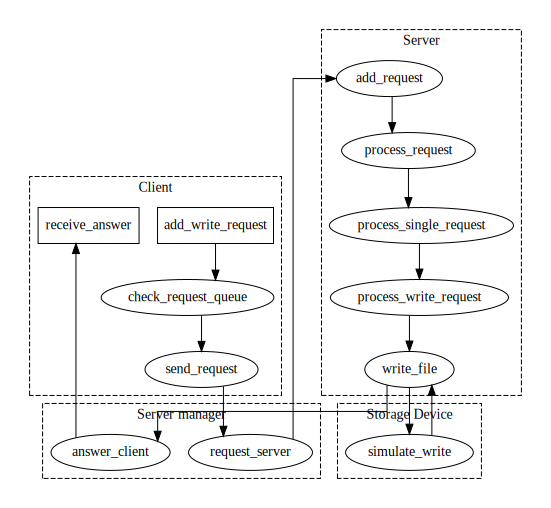
\includegraphics[width=\textwidth]{map.png}
The picture capture a possible configuration of IME:
\begin{itemize}
    \item 3 Clients with a single HDD each. These will generate the data that
        has to be stored in IME servers.
    \item a Network Fabric that interconnects every component of IME
    \item 2 SSDs per server, that can store data faster compared to the single
        client's HDD
\end{itemize}

Given the skeleton of the architecture, can be added or removed clients,
servers and disks for each one. This changes will end in different performances
that the simulator must be able to detect. \\
Part of the work is to inspect also different system layouts. The advantage of a
simulator is the ability to ensure the quality of a layout without the need to
test it for real, assuming the simulator is precise enough.
Every layout will be discussed in depth in the analysis section
(\ref{sys-analysis}).

\subsection{Network communication time}\label{netbuff}
Network communication is one of the main task that are committed in this system,
so we need an accurate model to represent it. \\
The parameters that determine the time elapsed in a network transaction are
\textit{latency} and \textit{bandwidth}. A file in theory is sent dividing
its size by the bandwidth available. In the real world we have to keep account also
the latency present inside the system: the smallest file will be sent
only after $<latency>$ amount of time. \\
From \cite{packet-size-ib} we know that the optimal packet size for
communication over infiniband is 1MB. \\
IME Client packs together requests smaller than this threshold and split bigger
files to achieve this communication pattern. This is further referred as
\textbf{Network Buffer}.  If requested explicitly, every request can be flushed
in order to complete a communication in case of remainders.  This set a domain
over the size of the packet sent: we always will have packets that are in the
interval $]0, 1024] KB$. The model should predict correctly the time required by
any network communication inside this interval. \\ In this case the only bond I
have are the 2 coordinates \\

\vspace{0.5cm}
\begin{tabular}{c | c}
    file size (KB) & time required \\ \hline
    0 & \textit{latency} \\ \hline
    1024 & \textit{1024KB / bandwidth}
\end{tabular}
\vspace{0.5cm}

These are respectively the worst and the best usage of the network. \\
I can obtain a more accurate model running some benchmarks on IME network, but
from a starting point I can rely on these 2 constraint. \\
Having the possibility to choose my interpolating function, I decided to use a
function with a diagonal limit, namely $\lim_{x \to +\infty} y(x) = +\infty$, that is a real behaviour
for every network. \\
The function of choice then is an \textit{hyperbole} adjusted to match the
specified coordinates. \\
\includegraphics[width=\textwidth]{diaglimit.png}


\subsection{Tokenized communication}
\subsection{Erasure coding for data loss} \label{pargroup}
In CPU caches, whenever happens a cache miss, data is read from main memory
instead. No data can be potentially lost. In the worst case cache won't be
useful. \\
IME acts as a cache too but for the problem it is solving, there is no
communication between the source and the target. This means that if data
is lost inside IME, it is \textit{permanently} lost. IME has a system to overcome this
problem that is \textit{Erasure Coding}. \\
As it happens in RAID level 4, 5 and 6, what is stored in the disks is not just
data but also an added amount of data based on the original data. In case of
loss of one piece of data, this missing part can be reconstructed comparing
remaining data and parity. \\
\includegraphics[width=\textwidth]{raid-level4.jpg} \\
For this correction system to work, we need to make associations between groups
of data that must be grouped together later when data loss happens. IME
considers a single block of data a Network Buffer (see \ref{netbuff}) and the
group that will contribute to data recovery as a \textbf{Parity Group}. \\
As an example, from the picture A1, A2, A3 and A$_p$ are individually a Network
Buffer. All of them grouped together makes a Parity Group. \\
The parity is generated by the client since the servers has only to keep track
about their status. \\
Is essential that every piece of that of the same parity group are sent to
different server: the loss of a single server could otherwise means the loss of
multiple piece of data. If every part is stored in a different server, the
inactivity of a single machine is not a fatal error for the system.
Is worth highlighting that with this approach bigger files are spread easier
inside the system, so every resource is exploited as much as it can.

\newpage

\subsection{Server Side file management}
From the client point of view, a server is a single block of storage. Actually
inside a single server is there are many disks that holds data and their
metadata. A client should only track the location of its stored files, in order
to not performing a broadcast on the network looking to read them. 
\footnote{Clients perform request of size 1MB. Parity groups are chosen in a
pseudo-random way in order to distribute the load to exploit better the
resources. If a file is big enough so that it is written to all the servers,
what happens is actually a broadcast, but for smaller files this technique is
effective} \\
On server side, to maximize performance, every disk should be used for data
storage. Hence the single request is split into smaller parts called
\textit{CML\_oid} with size of 128KB at maximum. \\
These data structure is only an abstraction over single files. CML\_oid-s are not
related to files but are closer to byte streams: every 128 KB of data a CML\_oid
is created containing completely or partially a file. \\
\vspace{0.5cm}
\includegraphics[width=\textwidth]{cmloid.png} \\
In the picture, the upper colored layer represent the files that are packed inside
a request. Each of them has different dimension to better show this approach.
Server now consider this request as a byte stream splitting it in slices of 128
KB, a CML\_oid. Every CML\_oid is then sent to a different server in a
round-robin fashion to distribute the load.

\subsubsection*{}
Moreover, because of the way an HDD works, there is a lower minimum size it can
interact with. If the user wants to edit a single byte on the file system, the
HDD will read a bigger amount of data, accept user modification, and write again
the bigger amount of data. If this amount of data is 256KB, for instance,
performing 8 write of 256KB or 1B each, will result in the same performances.
The only difference is that, if we are aware of this fact, we can make use of it
writing 2MB instead of 8B respectively.

\subsection{IO operations}
IME supports different IO operations depending on the task
\begin{itemize}
    \item \textbf{Sync}: the content of IME is copied to the mass storage, in
        order to have 2 copies of it. \\
        An use case can be keeping a remote file consistent to be read from
        others server later, leaving the chance to edit it later on IME.
    \item \textbf{Purge}: the files on IME are moved to the mass storage, not
        leaving any data on IME server. \\
        An use case is making some space because the disk is too filled, making
        space for some other data.
    \item \textbf{Erase}: files on IME are deleted, not making more copies of
        them. \\
        Happens when the data stored are just temporary, so there is no need to
        propagate further in the system.
\end{itemize}

These operations will be implemented in the simulator as well in order to better
classify the models. The objective is to test a model against a set of these
operations and extracting some measure to classify it.
